\documentclass{article}
\usepackage{amsmath}
\usepackage[margin=3cm]{geometry}
\usepackage{pgfplots}

\begin{document}

\title{History/inertia modeling terms}
\author{M. West}
\date{2013-12-26}
\maketitle

\section{Definitions}

\begin{center}
  \begin{tabular}{ll}
    $i$ & user number \\
    $j$ & question number \\
    $P_{ij}$ & predicted probability that user $i$ will get question $j$ correct \\
    $f_{ij}$ & intrinsic (non-historical) question response function \\
    $N_{ij}$ & number of times that user $i$ has attempted question $j$ \\
    $C_{ij}$ & number of correct answers by user $i$ for question $j$ \\
    $R_{ijk}$ & outcome of attempt $k$ by user $i$ on question $j$ (1 is correct, 0 is incorrect) \\
    surprise & average of $-p_k \log p_k$ where $p_k$ is the predicted probability of each event that occurred \\
    accuracy & fraction of correctly predicted (maximum likelihood) outcomes
  \end{tabular}
\end{center}

\begin{align*}
  f_{ij} &= \gamma_j + \frac{\delta_j (1 - \gamma_j)}{1 + \exp(-\alpha_j^T \sigma_i - \beta_j)}
\end{align*}

\section{Interpolate to total average by number of attempts}

\begin{align*}
  P_{ij} &= \epsilon_{ij} f_{ij} + (1 - \epsilon_{ij}) A_{ij} \\
  \epsilon_{ij} &= \exp(-\lambda N_{ij}) \\
  A_{ij} &= \frac{C_{ij}}{N_{ij}}
\end{align*}

\begin{center}
  \begin{tabular}{lll}
    $\lambda$ & surprise & accuracy \\
    \hline
    1 & 0.7686668964497944 & 0.6347603319783198 \\
    0.1 & 0.6272702026228207 & 0.6528836382113821 \\
    0.01 & 0.6220149300149277 & 0.65673695799458 \\
    0.001 & 0.6238023689875576 & 0.6552760840108401
  \end{tabular}
\end{center}

\newpage
\section{Interpolate to weighted average by number of attempts}

\begin{align*}
  P_{ij} &= \epsilon_{ij} f_{ij} + (1 - \epsilon_{ij}) A_{ij} \\
  \epsilon_{ij} &= \exp(-\lambda N_{ij}) \\
  A_{ij} &= \frac{\sum_{k = 1}^{N_{ij}} w_{ijk} R_{ijk}}{\sum_{k = 1}^{N_{ij}} w_{ijk}} \\
  w_{ijk} &= \eta^{(N_{ij} - k)}
\end{align*}

\begin{center}
  \begin{tabular}{llll}
    $\lambda$ & $\eta$ & surprise & accuracy \\
    \hline
    0.1 & 0.9 & 0.6203041281655737 & 0.6612889566395664 \\
    0.1 & 0.8 & 0.6198438606324299 & 0.6626016260162602 \\
    0.1 & 0.6 & 0.6295738534807478 & 0.6604844173441734 \\
    0.1 & 0.4 & 0.6498283243089524 & 0.6503641598915989 \\
    0.01 & 0.9 & 0.6201348464898921 & 0.6587483062330624 \\
    0.01 & 0.8 & 0.6192763365827337 & 0.6593834688346883 \\
    0.01 & 0.6 & 0.6186751976305411 & 0.6589176829268293 \\
    0.01 & 0.4 & 0.618833100965304 & 0.6583036924119241
  \end{tabular}
\end{center}

\newpage
\section{Interpolate to maximum by number correct}

\begin{align*}
  P_{ij} &= \epsilon_{ij} f_{ij} + (1 - \epsilon_{ij}) \delta_j (1 - \gamma_j) \\
  \epsilon_{ij} &= \exp(-\lambda C_{ij})
\end{align*}

\begin{center}
  \begin{tabular}{lll}
    $\lambda$ & surprise & accuracy \\
    \hline
    1 & 0.6198403173009505 & 0.6663490853658537 \\
    0.6 & 0.6169126483929738 & 0.6667513550135501 \\
    0.5 & 0.6159732081919393 & 0.667894647696477 \\
    0.4 & 0.61494345283247 & 0.6683604336043361 \\
    0.3 & 0.6138971928583951 & 0.6693131775067751 \\
    0.2 & 0.6131486865437922 & 0.6700330284552846 \\
    0.14 & 0.613231771872594 & 0.6670689363143631 \\
    0.1 & 0.6139487267351179 & 0.6659468157181572 \\
    0.09 & 0.6142748879805409 & 0.6652057926829268 \\
    0.08 & 0.6146749274245235 & 0.6645918021680217 \\
    0.01 & 0.6216176574174409 & 0.6593199525745257
  \end{tabular}
\end{center}

\begin{center}
  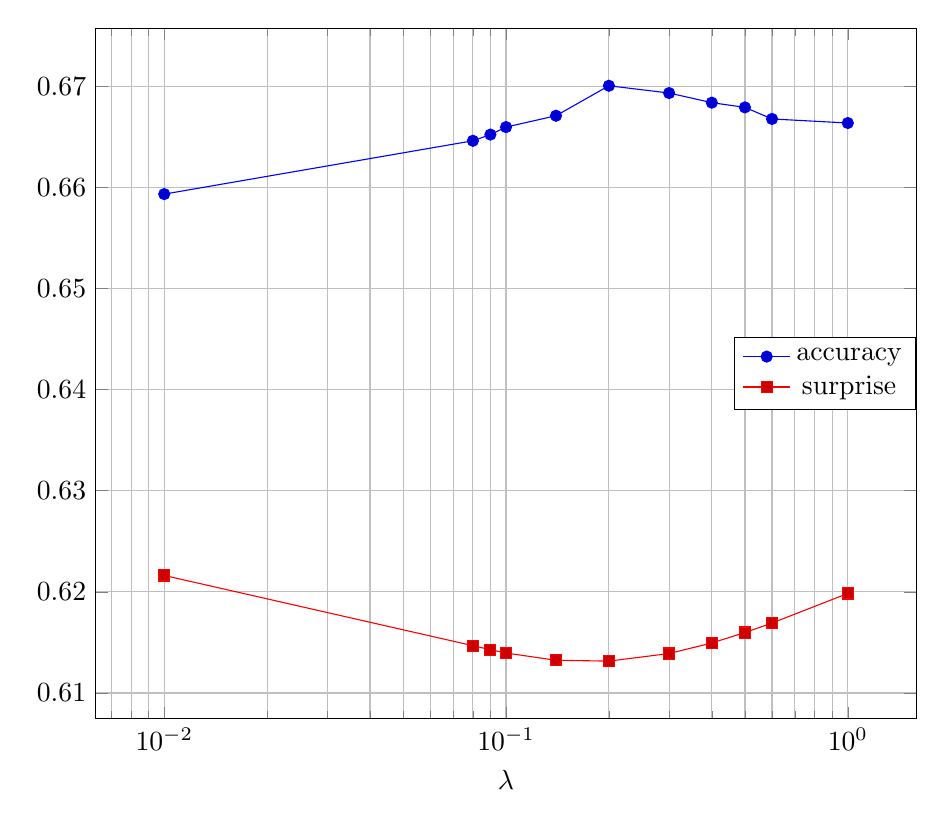
\begin{tikzpicture}
    \begin{semilogxaxis}[
      width=12cm,
      grid=both,
      xlabel={$\lambda$},
      legend style={at={(1,0.5)},anchor=east}
      ]
      \addplot coordinates {
        (1,0.6663490853658537)
        (0.6,0.6667513550135501)
        (0.5,0.667894647696477)
        (0.4,0.6683604336043361)
        (0.3,0.6693131775067751)
        (0.2,0.6700330284552846)
        (0.14,0.6670689363143631)
        (0.1,0.6659468157181572)
        (0.09,0.6652057926829268)
        (0.08,0.6645918021680217)
        (0.01,0.6593199525745)
      };
      \addlegendentry{accuracy};
      \addplot coordinates {
        (1,0.6198403173009505)
        (0.6,0.6169126483929738)
        (0.5,0.6159732081919393)
        (0.4,0.61494345283247)
        (0.3,0.6138971928583951)
        (0.2,0.6131486865437922)
        (0.14,0.613231771872594)
        (0.1,0.6139487267351179)
        (0.09,0.6142748879805409)
        (0.08,0.6146749274245235)
        (0.01,0.6216176574174409)
      };
      \addlegendentry{surprise};
    \end{semilogxaxis}
  \end{tikzpicture}
\end{center}

\newpage
\section{Interpolate to maximum by number correct, question-dependent}

\begin{align*}
  P_{ij} &= \epsilon_{ij} f_{ij} + (1 - \epsilon_{ij}) P_{\text{max}} \\
  \epsilon_{ij} &= \exp(-\exp(\lambda_j) C_{ij})
\end{align*}

Initial condition for $\lambda_j$ is mean -1.6, standard deviation 0.4.

\begin{center}
  \begin{tabular}{lll}
    $P_{\text{max}}$ & surprise & accuracy \\
    \hline
    $\delta_j (1 - \gamma_j)$ & 0.6117489909501538 & 0.670117716802168 \\
    $\delta_j (1 - \gamma_j) + \gamma_j$ & 0.6141570024189854 & 0.6704352981029811 \\
    $1$ & 0.6182441360920535 & 0.6679369918699187
  \end{tabular}
\end{center}

\begin{center}
  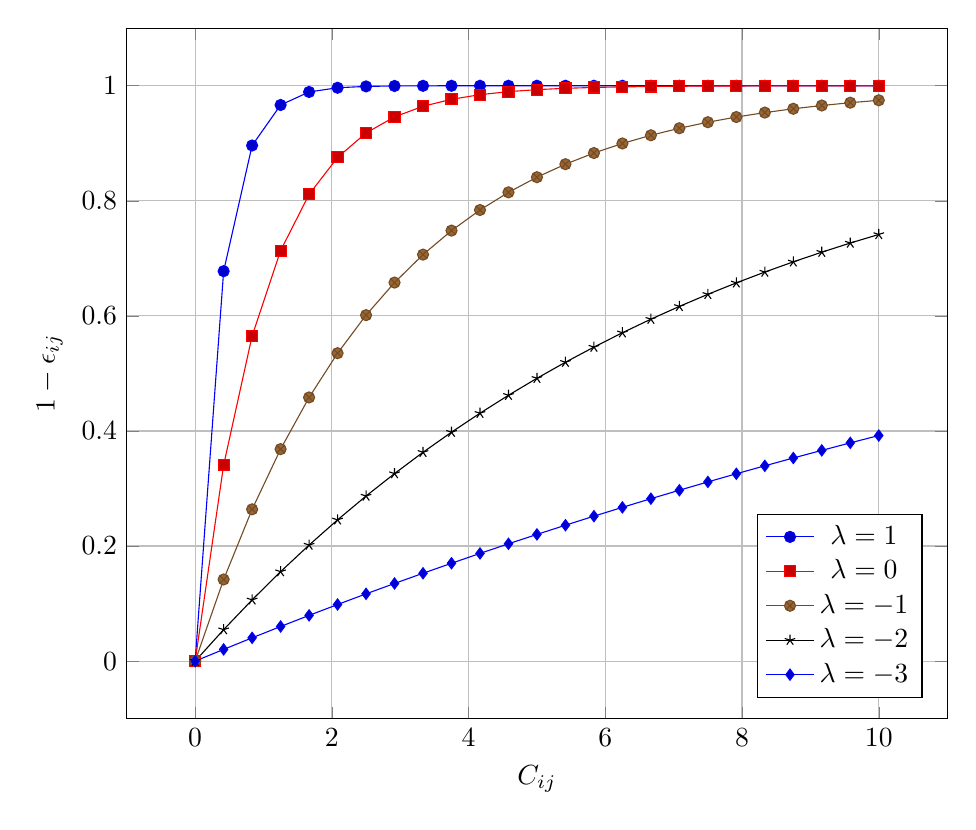
\begin{tikzpicture}
    \begin{axis}[
      width=12cm,
      grid=both,
      xlabel={$C_{ij}$},
      ylabel={$1 - \epsilon_{ij}$},
      domain=0:10,
      legend pos=south east
      ]
      \addplot {1 - exp(-exp(1) * x)};
      \addlegendentry{$\lambda = 1$};
      \addplot {1 - exp(-exp(0) * x)};
      \addlegendentry{$\lambda = 0$};
      \addplot {1 - exp(-exp(-1) * x)};
      \addlegendentry{$\lambda = -1$};
      \addplot {1 - exp(-exp(-2) * x)};
      \addlegendentry{$\lambda = -2$};
      \addplot {1 - exp(-exp(-3) * x)};
      \addlegendentry{$\lambda = -3$};
    \end{axis}
  \end{tikzpicture}
\end{center}

\newpage
\section{Dynamic model}

Assume normal distribution for $\sigma_i$:
\begin{align*}
  \sigma_i^t &\sim N(\mu_i^t, \Sigma_i^t)
\end{align*}
Dynamic update:
\begin{align*}
  \mu_i^{t+1} &= \mu_i^t \\
  \Sigma_i^{t+1} &= \Sigma_i^t + \nu\,\text{Id}
\end{align*}

\begin{center}
  \begin{tabular}{lll}
    $\nu$ & surprise & accuracy \\
    \hline
    0.1 & 0.6161413534818716 & 0.6677464430894309 \\
    0.01 & 0.6136431012186715 & 0.6694402100271003 \\
    0.001 & 0.6136773526542418 & 0.6699483401084011 \\
    0.0001 & 0.6140631452362125 & 0.670604674796748
  \end{tabular}
\end{center}

\newpage
\section{Modeled interpolation, binary}

Binary state $\epsilon_{ij}$ is 1 if user $i$ has no special knowledge
of question $j$, and is 0 if this user has figured out how to do that
question.
\begin{align*}
  P_{ij} &= \epsilon_{ij} f_{ij} + (1 - \epsilon_{ij}) (\delta_j (1 - \gamma_j) + \gamma_j)
\end{align*}
Initial distribution is $E[\epsilon_{ij}] = \epsilon_0$.

\begin{center}
  \begin{tabular}{lll}
    $\epsilon_0$ & surprise & accuracy \\
    \hline
    0.99 & 0.6237286861758857 & 0.6553396002710027 \\
    0.98 & 0.6237979249567114 & 0.6554878048780488 \\
    0.95 & 0.6244160499154667 & 0.6548949864498645
  \end{tabular}
\end{center}

\section{Modeled interpolation, continuous}

State $\epsilon_{ij}$ is in $[1,0]$, with an assumed beta
distribution.
\begin{align*}
  P_{ij} &= \epsilon_{ij} f_{ij} + (1 - \epsilon_{ij}) (\delta_j (1 - \gamma_j) + \gamma_j)
\end{align*}
Initial distribution has:
\begin{align*}
  \operatorname{E}[\epsilon_{ij}] &= \epsilon_0 \\
  \operatorname{Var}[\epsilon_{ij}] &= 0.9 \epsilon_0 (1 - \epsilon_0)
\end{align*}

\begin{center}
  \begin{tabular}{lll}
    $\epsilon_0$ & surprise & accuracy \\
    \hline
    0.99 & 0.6234936612091059 & 0.6558053861788617 \\
    0.95 & 0.6236469017659542 & 0.6554454607046071
  \end{tabular}
\end{center}

\newpage
\section{Conclusions}

\begin{enumerate}
\item None of the various schemes perform substantially better than
  the others in terms of minimizing average surprise or maximizing
  average accuracy.
\item If the aim is to stop students gaining benefit by repeatedly
  answering one question that they can do correctly, then it will be
  sufficient to use any of the schemes that interpolate to a constant
  based on number of attempts or correct answers.
\item The value of the constant to interpolate to is not very
  important, and can be $P_{\text{max}}$ or some average of outcomes.
\item To encourage spaced-repetition learning, the interpolation
  factor can also be a time-weighted function of the number of
  attempts. For example:
  \begin{align*}
    \epsilon_{ij} &= \exp(-\lambda E_{ij}) \\
    E_{ij} &= \sum_{k = 1}^{N_{ij}} \exp\left(\frac{t_{ijk} -
        t_{\text{now}}}{\tau}\right)
  \end{align*}
  where $t_{ijk}$ is the time of attempt $k$ by user $i$ on question
  $j$, $t_{\text{now}}$ is the current time, and $\tau$ is a
  characteristic decay time. Reasonable values would be $\tau = 1\rm\
  day$ and $\lambda = 0.3$.
\item Rather than using actual true time as the weighting, we could
  also use a per-user sequence number, so that doing other questions
  builds up the sequence number. For example:
  \begin{align*}
    \epsilon_{ij} &= \exp(-\lambda E_{ij}) \\
    E_{ij} &= \sum_{k = 1}^{N_{ij}} \exp\left(\frac{S_{ijk} -
        S_i}{S_{\text{decay}}}\right)
  \end{align*}
  where $S_{ijk}$ is the sequence number of attempt $k$ by user $i$ on
  question $j$, $S_i$ is the current sequence number for user $i$, and
  $S_{\text{decay}} = 20$ is a characteristic scale.
\end{enumerate}

\end{document}
